This chapter describes the implementation details of the JS-QL framework and language, as presented in chapter \ref{ch:JSQL}. The implementation of JS-QL is publicly available\footnote{https://github.com/voluminat0/Jipda-Security} and can freely be used to test source code for characteristics and vulnerabilities.


\section{Architecture}
The architecture of the implementation separates each component in a different module, providing the possibility to replace these modules by alternative implementations. In this section we discuss what each component represents.

\subsection*{Datastructures}
The \texttt{DataStructures} module defines all datastructures used in JS-QL. These include all kinds of tuples used for our matching algorithm, but also the alternative representations of edges and nodes to transform the abstract state graph to a compatible graph for the matching engine.

\subsection*{AbstractQuery}
The \texttt{AbstractQuery} module defines the core of the matching engine. It contains all operations on substitution sets: Matching, merging, defining extra properties, filters and lookups. The module provides an interface to the actual query algorithms \texttt{ExistentialQuery} and \texttt{UniversalQuery}, which perform the actual query matching processes.

\subsection*{Automaton}
The \texttt{Automaton} module defines the uniform representation of finite state machines (also known as finite automatons). It abstracts away whether the automaton is a deterministic or non-deterministic automaton, and provides information about the accepting states and starting state of these automatons.

\subsubsection*{ThompsonConstruction}
The \texttt{ThompsonConstruction} module defines an algorithm to convert a regular expression to a NFA (non-deterministic finite automaton). It parses the regular path expression and adds zero or more states to the newly created automaton for each step in the parsing process.
\subsubsection*{SubsetConstruction}
The \texttt{ThompsonConstruction} module defines an algorithm to convert a NFA to a DFA (deterministic finite automaton). What this means is that it eliminates all $\epsilon$-transitions, which are transitions that can occur without reading an input symbol. The resulting automaton is used for both query algorithms.

\subsection*{JipdaInfo}
The \texttt{JipdaInfo} module transforms state information to a more readable format for users. This transformation is necessary to have enforce consistency in states representing an AST node. The transformed states are the actual states that are queried instead of the original JIPDA states.

\subsection*{JSQL}
The \texttt{JSQL} module defines the internals of the JS-QL query language. It is implemented as an embedded DSL in JavaScript and allows users to define application-specific predicates and policies. The module is made available for the user through a fluent interface, increasing the readability of the language.

\subsection*{SecurityAnalysis}
The \texttt{SecurityAnalysis} module glues every component together in the framework. The initialization and transformation of the abstract state graph, execution of queries and processing query results are all invoked by this module.

\section{The user interface}
The JIPDA analysis comes packed with an interface which enables the user to inspect the abstract state graph. This state graph is generated when the user provides an input program and a lattice to perform the abstract interpretation. For our framework we augmented this user interface in several ways described in this section. Figure \ref{fig:UI} shows the user interface, illustrating what we will discuss in the next sections.

\begin{figure}[h]
    \centering
      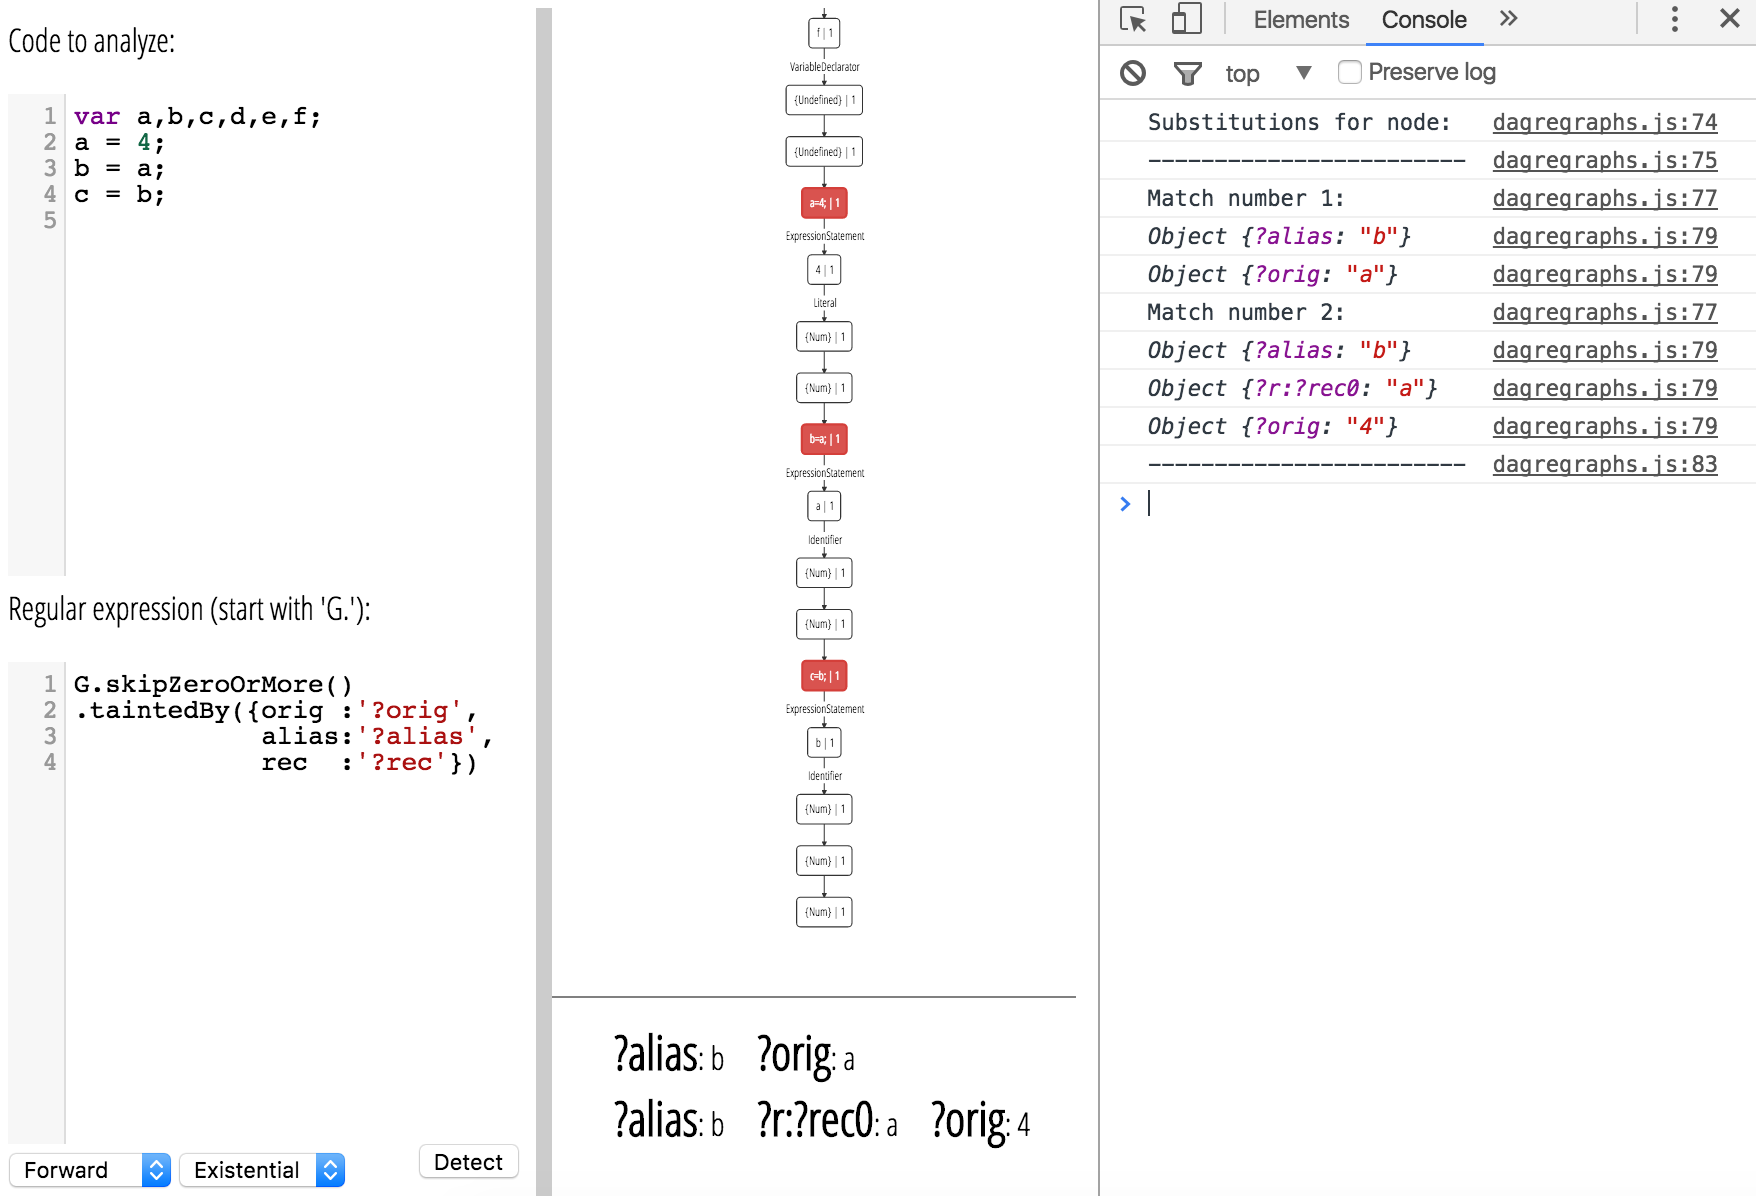
\includegraphics[width=1\textwidth]{images/UI} 
      \caption{The JS-QL framework user interface}
    \label{fig:UI}
\end{figure}

\subsection*{Query interpretation}

We decided to allow the user to specify queries in the user interface itself. In this way we avoid to switch between different screens and/or files to run just one query. The user interface contains a third-party JavaScript plugin which enables syntax highlighting. We use this plugin as input textboxes for a query and the input program. Along with entering the needed information, a user can decide the kind of query that needs to be executed. This can be done by selecting the direction together with type of query (existential or universal). When hitting the 'detect' button, internally a new \texttt{Query} object is made with the provided query string. Query objects contain three fields: The query direction, its type and a \texttt{JSQL} object, representing the instantiated query. Although being unsafe, the query string is converted to a JSQL object by \texttt{eval}uating it. For the sake of this dissertation, the safety of the application isn't relevant for its functionality.

\subsection*{The abstract state graph}

JIPDA already provided the functionality to display the abstract state graph in the user interface. In order to show results, this representation of the graph needed to be modified so that it became optimal for the user to reason about query results. We changed the following:
\begin{enumerate}
\item \textit{Edge labels}: The JIPDA state graph already contained edge labels, but the information they contained was irrelevant for our approach. As our approach uses edge labels to match states, we had to shift information from nodes to edges. All evaluation states' outgoing edges are also augmented with a visible edge label representing the type of AST node it contains, to make it easier for the user to see what he has to specify in his queries.
\item \textit{State colours}: The default colours of all JIPDA states have been stripped from the graph. This was done to increase the contrast with marked states (i.e. states indicating a match of the query). When the matching engine produced all results, these results have to be transferred to the corresponding states of the state graph. A 'marker' property was added to each matched state, containing the match information as well as a CSS class to highlight them in the otherwise colourless graph. This CSS class can be customised by the user.
\end{enumerate}

\subsection*{Results inspection}

Each query result is a set of substitutions, mapping variables (denoted by a starting \texttt{?}) to their corresponding values in the state graph. Every matching state is marked with its substitution set(s). These results can then be further explored through the results section under the state graph or in the browser's built-in console, which allows to inspect results in even greater detail.


\section{The query language}
\label{sec:queryLanguageImpl}
The JS-QL query language is implemented as an embedded DSL with JavaScript as its host language. We motivated the use of a DSL in chapter \ref{ch:Overview} and explored the JS-QL syntax and semantics in chapter \ref{ch:JSQL}. This section describes how the DSL is implemented and how we incorporated several DSL implementation techniques.

A JS-QL query gets parsed like a regular expression. Each state in the pattern represents one character in the regular expression, defined by objects of type \texttt{RegexPart}. These parts of the pattern have 5 fields to ease the translation from regular expression to automaton:
\begin{enumerate}
\item \textit{Name}: The name of a regular expression part. In the current implementation, the name just denotes the type of the state/predicate that the \texttt{RegexPart} represents (e.g. \texttt{state, wildcard, not, lbrace, \ldots})
\item \textit{Symbol}: The actual symbol that will be parsed by the parser to set up the automaton corresponding to the query.
\item \textit{Object}: The argument of the state/predicate in which all variables are bound and properties, filters and lookups are specified.
\item \textit{ExpandFunction}: A higher order function representing a recursive predicate or policy that is called for recursive queries. This argument doesn't need to be specified when no recursion happens in a query.
\item \textit{ExpandContext}: A unique identifier to avoid overlapping recursive variable names. Only used for recursive queries.
\end{enumerate}

\noindent States and predicates are actually just function calls returning \texttt{this} to enable method chaining (which is a commonly used technique to implement a fluent interface). Each function call actually represents one state in the pattern, and thus for each of these calls the corresponding \texttt{RegexPart} gets pushed into a map containing the pattern information. 
An exception to this are recursive queries. Recursive query patterns can have an arbitrary amount of states, so we can't model them directly as a sequence of \texttt{RegexPart}s as we don't know the length of the actually matched pattern. We therefore store a whole recursive query in just one \texttt{RegexPart} object, and mark it with 'subgraph' as its name. Further we specify the \texttt{ExpandFunction} and \texttt{-Context} to be able to process the subgraph in the matching algorithm. The idea for treating recursive queries like was adopted from the PQL language\cite{PQL}. The information in this map is unmodified in the sense that the variables aren't resolved yet. The entire query pattern (i.e. the map) is then processed by applying \textit{Thompson's Construction Algorithm} and the \textit{Subset Construction Algorithm} consecutively to obtain a NFA and DFA respectively. These algorithms won't be discussed in too much detail, as they are well described in many online resources and in the literature\cite{Thompson}. An overview of how queries are processed is depicted in figure \ref{fig:QueryProcessing}.

\begin{figure}[!h]
    \centering
      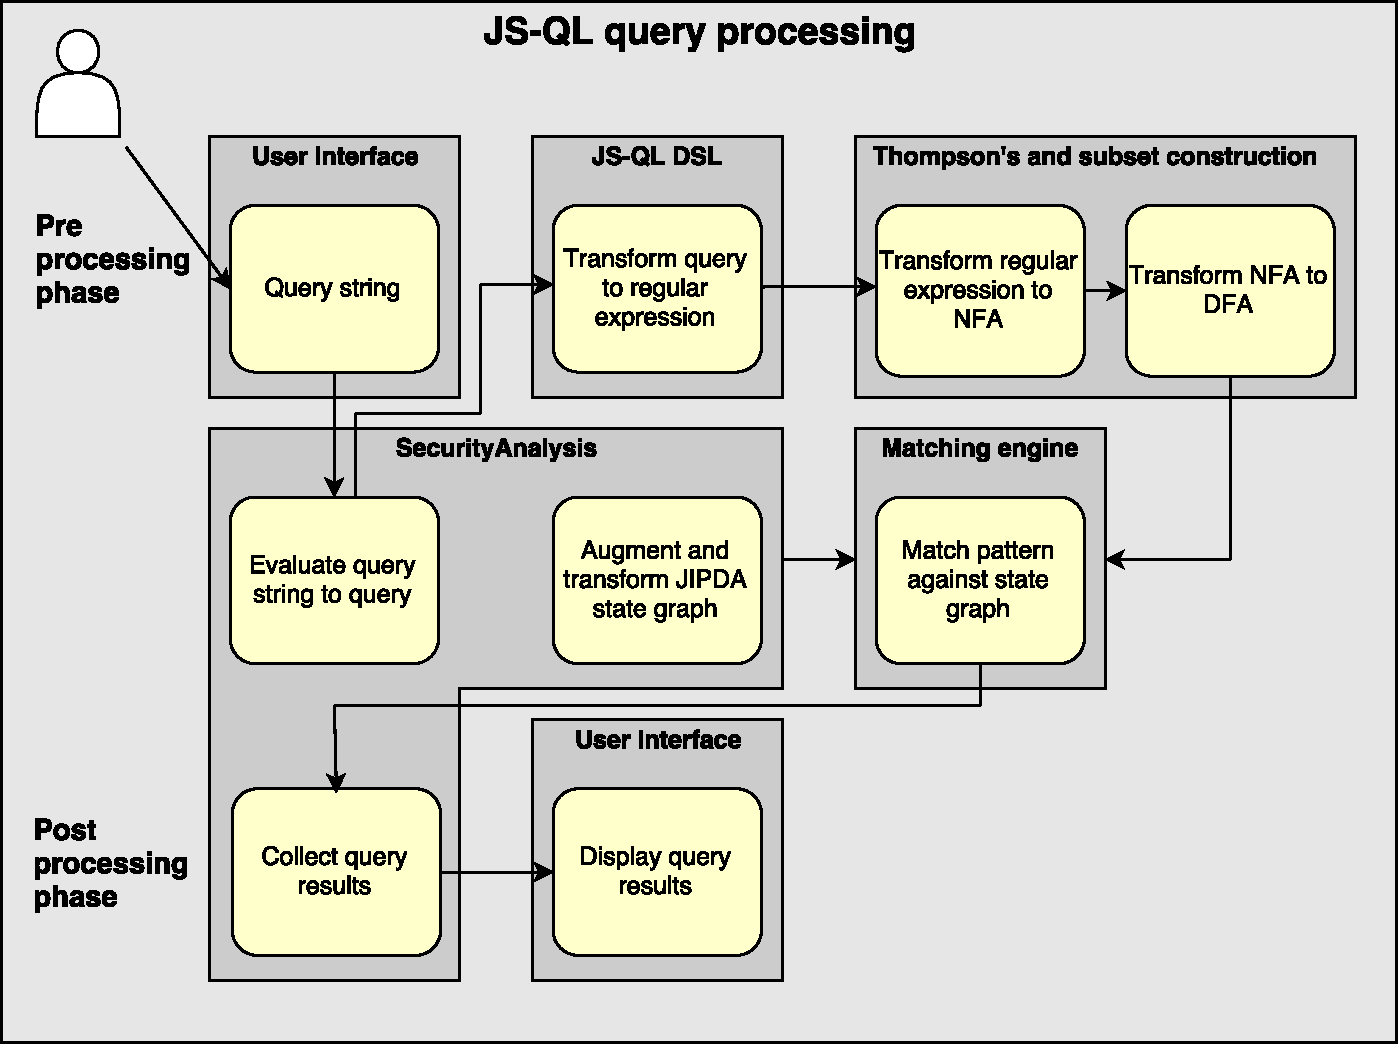
\includegraphics[width=1\textwidth]{images/QueryProcessing} 
      \caption{Stages of processing a query}
    \label{fig:QueryProcessing}
\end{figure}

\subsection*{Regular, temporary and recursive variables}

JS-QL supports three types of variables: Regular, temporary and recursive variables. Each of these types of variables has its own function in the framework:
\begin{enumerate}
\item \textit{Regular variables}: These variables contain the information that the user wants to match in a query. When a match succeeds, they will always be contained in the resulting substitutions.
\item \textit{Recursive variables}: Variables that are used as intermediary variables. They function as a variable that was bound in the previous step of a recursive query, enabling a recursive step to work with the value of one or more variables of the previous step. The \texttt{taintedBy} example used in chapter \ref{ch:JSQL} uses a recursive variable to store all intermediary assignments.
\item \textit{Temporary variables}: These variables are state-local. They are used when a user doesn't specify a certain argument for a predicate or policy. When only specifying the \texttt{left} argument for the \texttt{assign} predicate shown in chapter \ref{ch:JSQL}, the \texttt{right} and \texttt{this} will be bound to temporary variables. These variables get dropped from the resulting substitutions.
\end{enumerate}

\noindent By allowing the user to choose from three types of variables, writing queries becomes very flexible. In this way the bindings in a substitution set can be limited to only the information needed by the user. When imagining JS-QL without the support of temporary variables for example, the size of the substitution set for more complex queries would grow very large very quickly. This greatly decreases the readability of the results and makes interpretation of these results much harder.

\subsection*{Deferring evaluation of properties and filters}

One way to define properties is to use the \texttt{prop} function. Filters on the other hand can be expressed through the \texttt{cond} function. Both of these functions have one thing in common: The value they return depends on the value of the variables specified by the user. The problem now is that the value of these variables is not yet calculated at compile-time. Consider the following example: \texttt{cond('===', '?var', 3)}. Here, the state declaring \texttt{?var} is not yet matched in the state graph, meaning that \texttt{?var} is not yet bound and that we can't check if it is equal to 3. We remedy this by deferring the evaluation of the specified function. Instead of passing the result of evaluating the function directly with its arguments, we wrap them into a \textit{thunk} and pass that thunk to the matching engine. When the matching engine finally needs the value of the thunk, it unwraps it and resolves all variables to the values to which they are bound. If not all variables are bound, the query fails.

\section{The matching engine}

The algorithms that are used as the base of the framework were first presented in \cite{algoEngine}. They discuss algorithms for matching regular path expressions with graphs containing simple information. These algorithms match the edge labels of the graph with the edge labels of the regular path expression (for the rest of dissertation, we will call these expressions \textit{pattern}s). For our implementation, this already formed 3 obstacles:
\begin{enumerate}
\item \textit{Subgraphs}: Recursion can be a useful tool for certain analyses based on queries. The algorithms presented don't support recursion, and thus don't provide constructs for recursive queries. We augmented these algorithms to consider subgraphs as a regular data structure and implemented a way to process them.
\item \textit{Information in edge labels}: The JIPDA state graph is built as a sort of linked list of states. Each state contains information about itself but also has references to its successor states. Although this being only a minor obstacle, we had to find a way to transform the JIPDA state graph in such a way that all state information was available in the edges, instead of in the states. As no explicit edge information was available in the JIPDA state graph, we introduced a new type of graph representation containing tuples with a source state, an edge label (containing the source state information) and a target state. This graph representation is better suited to be processed by the algorithms.
\item \textit{Edge label information}: The information on the edge labels in the described algorithms consists of simple information. The arguments of a pattern can only be symbols, like a string or a literal, limiting the type of graphs that can be analysed. We remedy this by extending the algorithms to support nested maps as arguments, as these are the main datastructure in JS-QL for representing a state.
\end{enumerate}


In the remainder of this section we will discuss the core functionality of the matching engine. In section \ref{subsec:inputOutput} we briefly discuss the inputs and outputs of the matching engine. We then elaborate on the algorithms themselves in section \ref{subsec:algorithms}. All functionality used by these algorithms is discussed in sections \ref{subsec:matching}, \ref{subsec:merging} and \ref{subsec:subgraphs}. The flow of both algorithms is quite similar, and can be viewed in figure \ref{fig:matchingEngine}.

\begin{figure}[!h]
    \centering
      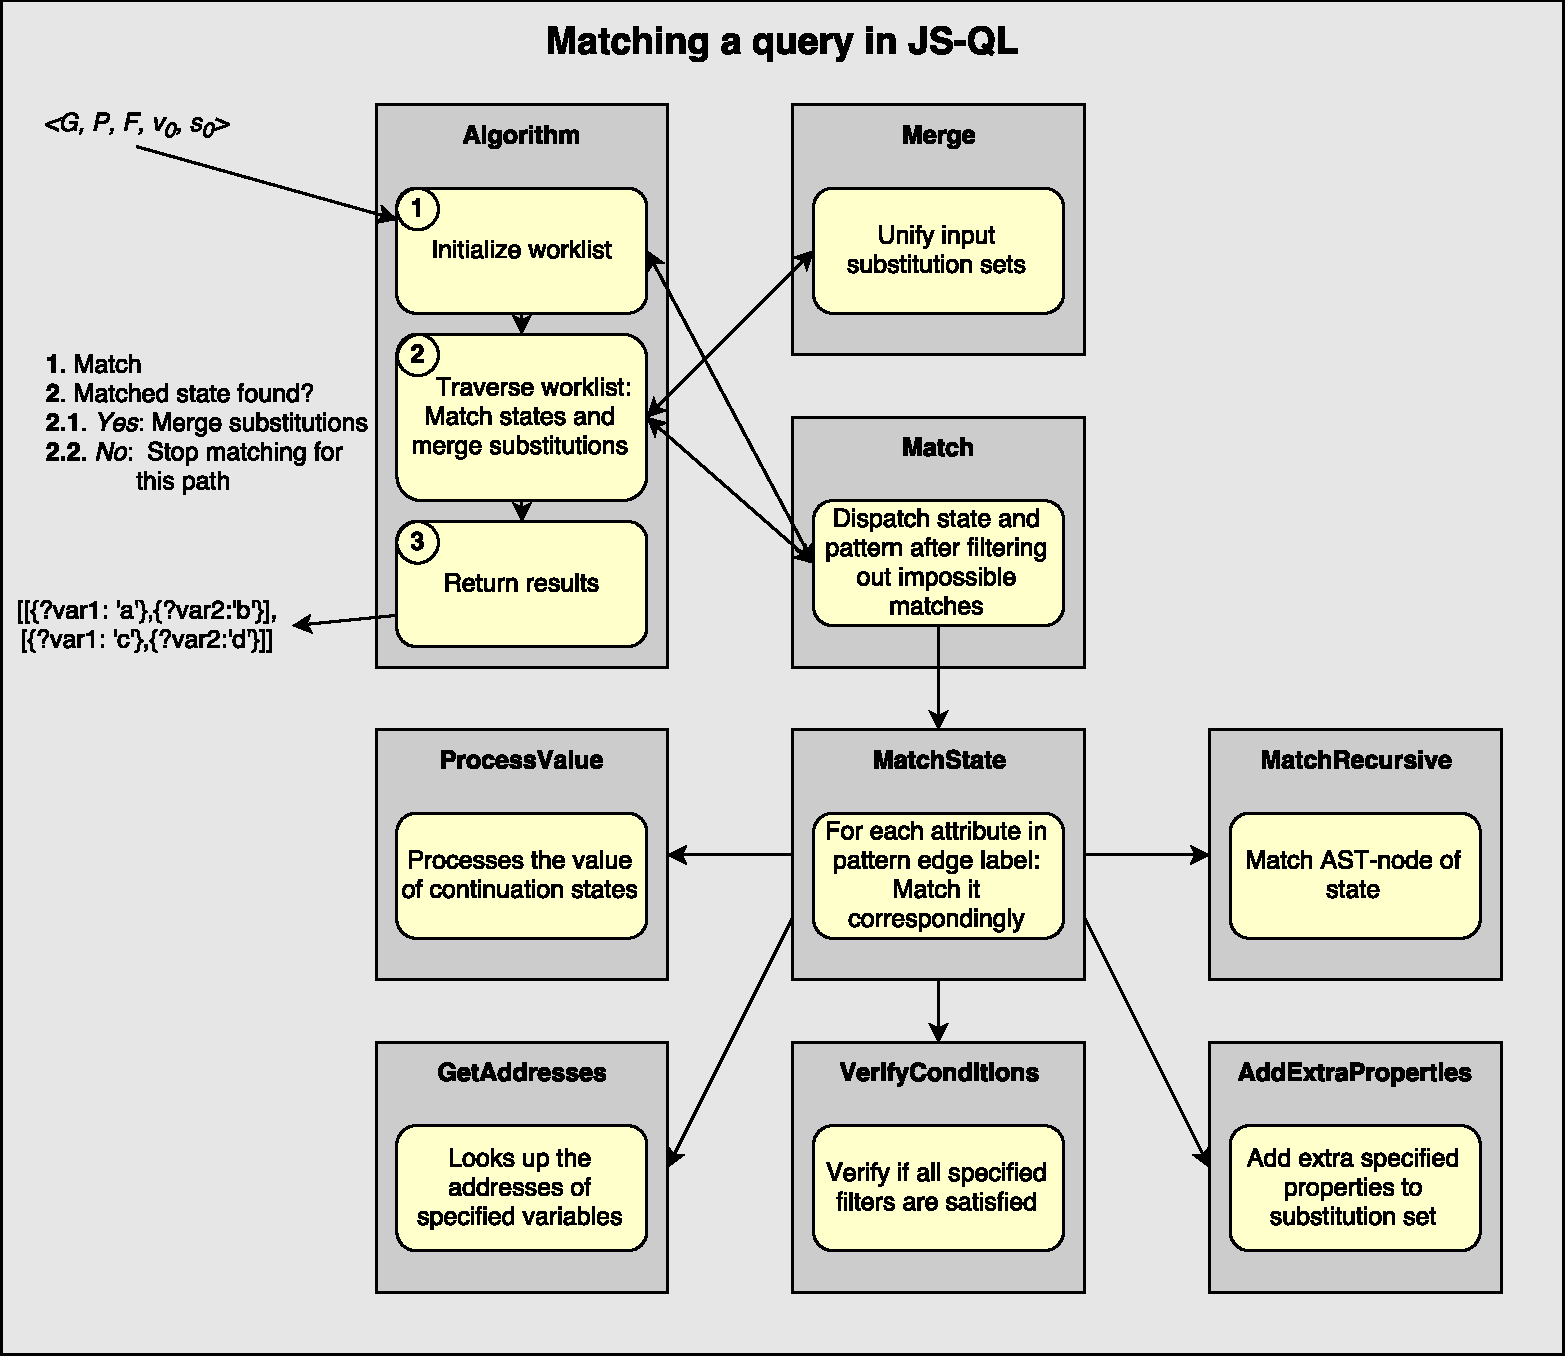
\includegraphics[width=1\textwidth]{images/matchingEngine} 
      \caption{Stages of matching a query}
    \label{fig:matchingEngine}
\end{figure}

\subsection{Inputs and output}
\label{subsec:inputOutput}
The inputs for both the existential query algorithm as the universal query algorithm are identical. In order to to match the state graph with a pattern, we have to provide them to the algorithm. The generated automaton for the pattern $P$ as well as the state graph $G$ are transformed to a uniform format, called \texttt{triples}. A triple in a pattern consists of two automaton states as source and target state and the edge between them, representing the part of state that needs to be matched (i.e. the nested map of state information). For the JIPDA state graph we transformed the original graph to a similar representation, as already described above. The final states $F$ of $P$ also need to be specified, so that the algorithm can determine when a match is completed and its substitutions can be added to the resultset. Finally the initial states of both the automaton ($s_0$) and the state graph ($v_0$) are also required, giving the algorithm an indication on where it should start matching. Together, this information forms the 5-tuple $<G, P, F, v_0, s_0>$.

The output of the algorithm is easier to explain. The results of the algorithm consists vertex-theta pairs, where a vertex is a state in the abstract state graph and theta is the set of all possible substitutions for the query ending in that state. In our implementation, we call these pairs \texttt{VertexThetaPair}s.

\subsection{Query algorithms}
\label{subsec:algorithms}

The internals of both algorithms can be divided into two main parts. The first part consists of initializing the worklist. This worklist $W$ contains triples of the form $<v, s, \theta>$, where $v$ is a state of the state graph, $s$ a state of the automaton and $\theta_s$ the set of substitutions that have been matched up until $s$ in the pattern. The algorithm loops over each state in the state graph to locate a triple $t_G$ in $G$ having the starting state $v_0$ as its source. Next, all triples in $P$ are traversed until initial state $s_0$ is found as the source state of a triple $t_P$. When both triples are found their edge labels are \textit{matched}. When the matching succeeds, a list of all possible substitutions $\theta$returned and the worklist gets updated to contain the destination states of $t_G$ and $t_P$ together with a substitution from $\theta$. Producing a match from two edge labels is discussed in section \ref{subsec:matching}. If no match between $v_0$ and $s_0$ is found, the query fails and no results are returned, as a match for the initial states can't be found anywhere in the state graph.

In the second phase of the algorithm, $W$ gets traversed. As already discussed, $W$ contains a state $v$ of the state graph, a state $s$ of the automaton and the partial match and substitution set $\theta$ between these two states. Each successor ($v_{succ}$ and $s_{succ}$) of both $v$ and $s$ are tried as the next match in a pattern, unless $s_{succ}$ is a state in the automaton representing a subgraph. If this is the case the pattern gets expanded, as will be explained in section \ref{subsec:subgraphs}. When a match is found, each found substitution $\theta_{succ_i}$between $v_{succ}$ and $s_{succ}$ gets merged with $\theta$. When this merge succeeds, the triple $<v_{succ}, s_{succ}, \theta_{succ_i}>$ is added to $W$, only if it hasn't already been processed in an earlier matching step, to prevent the algorithm from looping forever. This is called \textit{fixpointing}, and is applied by keeping track of the already reached triples in the reach list $R$. The merging process is descriped in more detail in section \ref{subsec:merging}. After the matching and merging process to acquire the next triple(s) for the worklist for a certain $v$ and $s$, the algorithm checks whether $s$ is contained in the list of final states $F$. When it does, a \texttt{vertexThetaPair} is added to the resultlist containing $v$, the state of the graph matching the final state of the pattern, and $\theta$, the set of all substitutions between $v_0$ and $v$. When the worklist is depleted no more paths need to be matched by the algorithm, indicating that all possible results have been collected. What rests is to return all \texttt{VertexThetaPair}s so that they can be processed in the user interface layer.
\\\\
\noindent The algorithm described is used to solve existential queries. Universal queries use an algorithm which is very similar, except for that it performs an extra check for the \textit{determinism condition} in the second phase of the algorithm. 
\begin{definition}
\textit{The \textbf{determinism condition} is a condition used in universal queries, imposing that for each path from $v_0$ to $v$ in $G$, all paths in $P$ that match it (under any substitutions) pass through the same set of states.}
\end{definition}
\noindent We implement this by setting a flag when a match is found for one path in $P$. If a match is found for another path in $P$, the determinism condition is violated and the matching engine halts execution. In this case, no results will be produced. Another condition for universal queries to produce results is that for each matching state in $G$, the corresponding state in $P$ is a final state. This last condition is rather trivial, as queries only produce a result if they are matched up until a final state.

\subsection{Matching states with a pattern}
\label{subsec:matching}

Matching in the strict sense of the word is checking if two things are equal. In our implementation, a match occurs when a state in $P$ is \textit{subsumed} by a state of $G$. What this means is that all the information that is contained in a state in the pattern has to occur in the state of the state graph that is currently being matched, allowing the latter to contain way more information than just what is specified by the pattern state. Figure \ref{fig:matchingPredicates} illustrates how a state is matched. The JS-QL predicate on the right produces a match, as it is subsumed by the JIPDA state. In contrast, the left JS-QL predicate specifies a \texttt{callee} attribute, which isn't contained in the JIPDA state. This suffices to produce a mismatch, leading to a failed match for the currently matched path in the state graph.

The JS-QL framework matches through the \texttt{match} function. This function is just an entry point to the matching process, as it only passes all matching work to the \texttt{matchState} function and waits for its results. \texttt{match} however does perform an initial check to make sure no excessive work is done. An example: When encountering a wildcard in the pattern, no matching needs to be done as a wildcard matches any state. Negation is also handled by this function: matching a negated pattern state simply consists of matching the regular state (i.e. the state without negation) and returning false when a match is found and the empty substitution list otherwise. The remainder of this section discusses the different phases of the matching process, as already has been depicted in figure \ref{fig:matchingEngine} above.

\begin{figure}[!h]
    \centering
      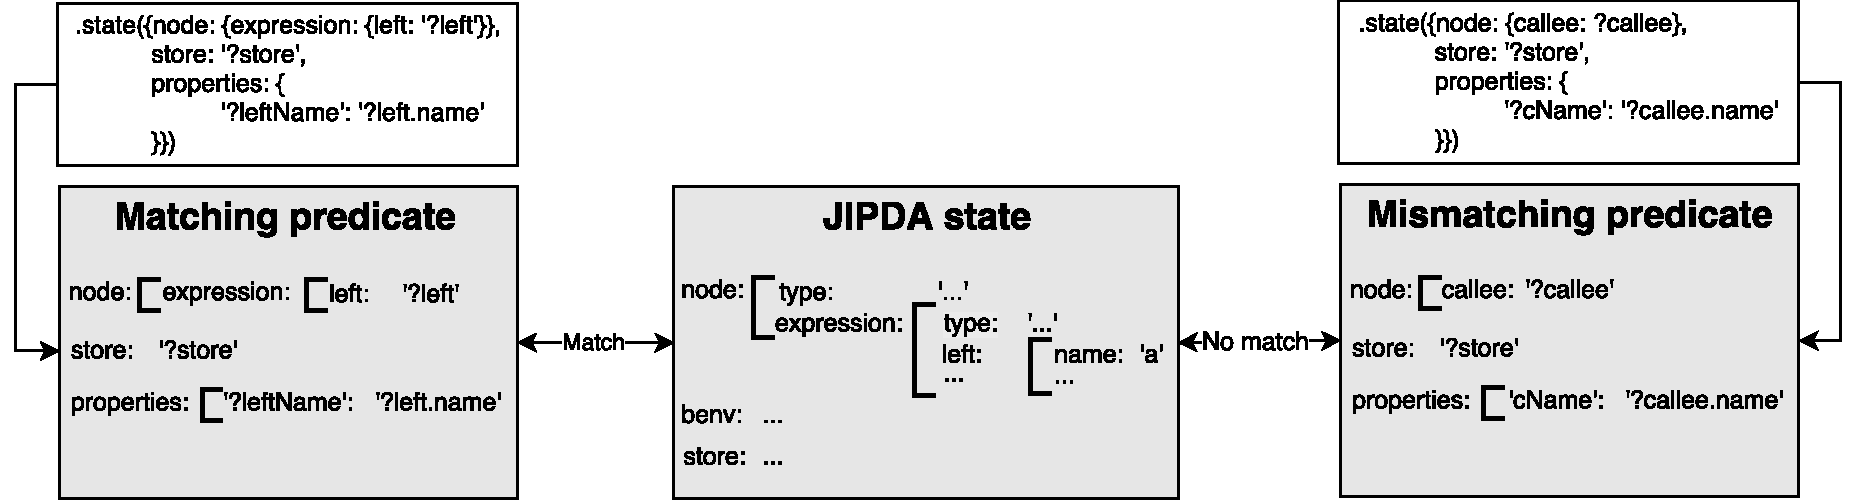
\includegraphics[width=1\textwidth]{images/matchingPredicates} 
      \caption{A matching and mismatching predicate for a JIPDA state}
    \label{fig:matchingPredicates}
\end{figure}

\subsubsection{matchState}
The \texttt{matchState} function is responsible for delegating the matching of keywords and combining the results of those matches. The initial substitution set $\theta$ is empty and grows larger for each keyword that is matched. Internally, the function works as follows: For each keyword specified in the JS-QL query, match its value (i.e. a nested map, a literal or a variable) with the corresponding attribute of the state to be matched and collect the results of this partial matching. If the partial match failed, \texttt{false} is returned, elsewise the partial match is merged with $\theta$. Each possible keyword has a different processing method (see figure \ref{fig:matchingEngine}), and we will briefly discuss each of them.

\subsubsection{matchRecursive}
The \texttt{node} attribute of states represents its corresponding AST node. This node gets matched recursively until a variable or a literal is encountered. In the case of a variable, the corresponding AST node value is bound to it. If each node-attribute of the predicate is matched, the substitution set containing all matched variables is returned. There are several reasons why the \texttt{matchRecursive} function would not produce a match:
\begin{enumerate}
\item As already mentioned, the AST node gets matched recursively until a variable or literal is encountered. In the case of a literal being matched, a mismatch occurs when the value of the literal doesn't agree with the value in the AST node.
\item In the other case, matching a variable which was already bound in a previous state results in a mismatch if the value of the variable can't be unified with the newly matched value.
\item The most common reason for a mismatch to happen is when a node-attribute specified in a JS-QL query isn't present in the AST node of a JIPDA state. This 'mismatching-technique' is often used instead of explicitly specifying the \textit{type} of the node in the predicate. Figure \ref{fig:matchingPredicates} illustrates this: The predicate on the right-hand side doesn't match as no 'callee' attribute is present in the current JIPDA state.
\end{enumerate}

\subsubsection{addExtraProperties}

This function matches the properties attribute of a predicate. The matching process is split in two, using one function for each way that properties can be defined: One function handles properties that just access attributes of already bound variables. The other function handles properties specified by \texttt{prop}. Both functions first resolve all needed variables, and fail to match if one or more variables can't be resolved (i.e. are not contained in the current substitution set). After resolving all used variables, the new variables defined by the properties are evaluated and added to the substitution set to be returned. \texttt{addExtraProperties} may produce no results if any of the same reasons as in \texttt{matchRecursive} occur.

\subsubsection{verifyConditions}

As the JS-QL language allows to express filters, a function is needed to evaluate and check these filters. \texttt{verifyConditions} does just that. Its internal working is very similar to the matching of properties. After resolving the needed variables, the specified filter function is applied to its arguments. When the condition for a filter holds, the next filter is checked. In the case that condition for a filter doesn't hold, the matching process is aborted. If all filters return \texttt{true} the matching process can continue, as the matched state meets all requirements that the filter imposes.

\subsubsection{getAddresses}
%Zoekt alle addressen op van een bepaalde naam. gebruikt hiervoor benv en store.
The \texttt{getAddresses} function looks up the addresses for the variable specified in the lookup map. Variables can have multiple addresses caused by precision loss due to abstract interpretation. For each name in the map, a literal or a variable to be resolved, the addresses are looked up using the binding environment and the store. When no address is found for the specified name (meaning that the variable doesn't exist at that point in the program), the matching process fails.

\subsubsection{processValue}
Continuation states all have a value attribute. This attribute contains the addresses or values for the expression or statement that has just been evaluated. The \texttt{processValue} function just duplicates the existing substitution set and adds one address/value to each of the duplicated substitution set. The resulting substitution sets each contain one possible value or address.



\subsection{Merging substitution results}
\label{subsec:merging}

%waarvoor dient merging
Merging happens when the substitution set of previously matched state in the pattern has to be combined with the newly acquired substitution set for the currently matched state. When these substitution sets can be combined, a valid next stap in the state graph is found with the newly created substitution set $\theta_{res}$. Else, the algorithm halts for the current path in the state graph, as the substitution sets can't be merged. Merging in the JS-QL framework is fairly straightforward. A merge between two substitution sets $\theta_i$ and $\theta_j$ only succeeds if no substitution of $\theta_i$ is contradicted by a substitution in $\theta_j$, and vice versa. When one substitution set contains a substitution that isn't contained in the other, the resulting substitution set will also contain that substitution. Two contradicting substitutions result in a mismatch, making the algorithm halt for the currently matched path. Table \ref{tab:merging} shows some possible outcomes of merging two substitution sets.

\begin{table}[!h]
\centering
  \begin{tabular}{| c | c | c |}
  \hline
  $\theta_i$ & $\theta_j$ & $\theta_{res}$\\
  \hline \hline
  %\{?var1: 'a'\}, \{?var2: 'b'\} & \{?var3: 'a'\} & \{?var1: 'a'\}, \{?var2: 'b'\}, \{?var3: 'a'\} \\
  ?var1: x & ?var3: x & ?var1: x\\
  ?var2: y &  & ?var2: y\\
  &  & ?var3: x\\
  \hline
  ?var1: x & ?var1: y & false\\
  \hline
  ?var1: x & ?var1: x & ?var1: x\\
  & ?var2: y & ?var2: y \\
  \hline

  \end{tabular}
  
  \caption{Examples of merging two substitution sets}
  \label{tab:merging}
\end{table}

\noindent The first example in the table succesfully merges the two sets because they are contain disjunct information. No overlaps in variables occur, so the resulting set is the union of both sets. A mismatch is encountered in the second example. The substitution value for \texttt{?var1} in $\theta_i$ differs from that in $\theta_j$, resulting in a failed merge. The last example again poses no problem to merge as \texttt{?var1} contains the same value in both sets and \texttt{?var2} is only contained in the second set.


\subsection{Processing subgraphs}
\label{subsec:subgraphs}

Recall that recursive query calls are represented in $P$ by a single state of type 'subgraph'. When encountered in an algorithm, this state has to be expanded in such a way that the pattern gets modified to contain \textit{one} additional recursive step. The algorithms used by JS-QL match a state of $G$ with a state of $P$, and halts the matching process for that path when no match is found. This has as a side effect that we indeed don't have to try and exhaustively expand each subgraph state, because the algorithm might never reach the expanded states. Another consideration is that if we were to expand the subgraph state multiple times, the algorithm might get trapped in an infinite loop as it doesn't know when to stop exploring recursive steps. Figure \ref{fig:subgraphExpansion} shows what happens when a recursive state of the \texttt{taintedBy} policy is encountered by the algorithms. We see that the subgraph in the original policy gets replaced by the entire pattern of that policy in the first recursive step.

\begin{figure}[!h]
    \centering
      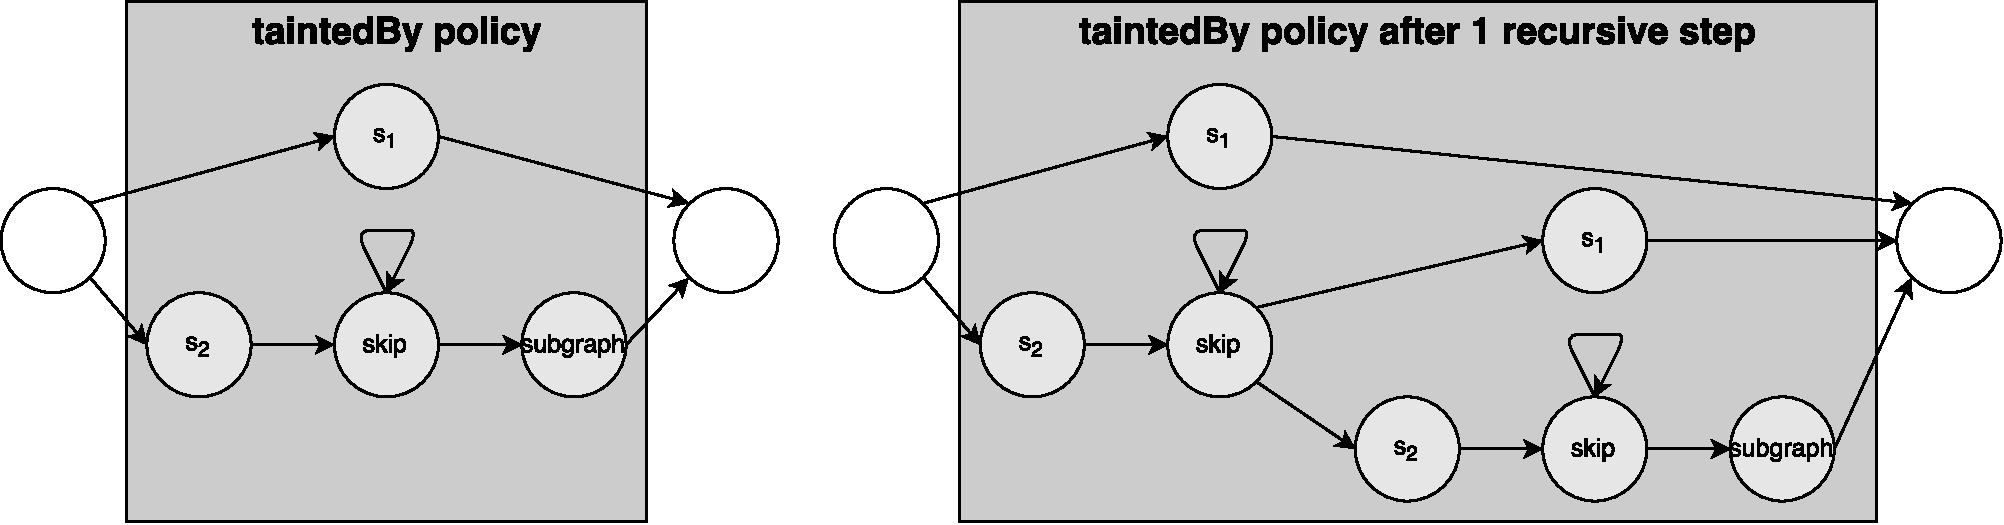
\includegraphics[width=1\textwidth]{images/subgraphExpansion} 
      \caption{Before and after expanding a subgraph for one recursive step}
    \label{fig:subgraphExpansion}
\end{figure}

Expansion of a subgraph state happens by applying the \texttt{expandFunction} (see section \ref{sec:queryLanguageImpl}), which is a predicate or policy returning a piece of a pattern $P_{subgraph}$, and replacing the subgraph state in $P$ by the obtained pattern $P_{subgraph}$. The same subgraph may be expanded for different paths in the state graph, resulting in costly computations for each of those paths. We remedy this by caching each expanded subgraph. A subgraph state (with its unique identifier) gets mapped to its expanded subgraph pattern. When in the next iteration of the algorithm a subgraph state is encountered, its corresponding subgraph pattern is first looked up in the cache. Only when there is no corresponding subgraph available, the subgraph will be calculated and added to the cache.




